% This is samplepaper.tex, a sample chapter demonstrating the
% LLNCS macro package for Springer Computer Science proceedings;
% Version 2.20 of 2017/10/04
%
\documentclass[runningheads]{llncs}
%
\usepackage{graphicx}
\usepackage{graphicx}
\usepackage{subfigure} 
% Used for displaying a sample figure. If possible, figure files should
% be included in EPS format.
%
% If you use the hyperref package, please uncomment the following line
% to display URLs in blue roman font according to Springer's eBook style:
% \renewcommand\UrlFont{\color{blue}\rmfamily}

\begin{document}
%
%\title{Tracing multiple neurons in  densely-packed microscopic images\thanks{Supported by organization x.}}
\title{Tracing multiple neurons in  densely-packed microscopic images}
%
%\titlerunning{Abbreviated paper title}
% If the paper title is too long for the running head, you can set
% an abbreviated paper title here
%
%\author{First Author\inst{1}\orcidID{0000-1111-2222-3333} \and
%Second Author\inst{2,3}\orcidID{1111-2222-3333-4444} \and
%Third Author\inst{3}\orcidID{2222--3333-4444-5555}}

\author{Peng Wang \and
Yimin Wang\and
Third Author}

%
\authorrunning{F. Author et al.}
% First names are abbreviated in the running head.
% If there are more than two authors, 'et al.' is used.
%
\institute{ShangHai University,CHINA\\
\email{wang\_peng@shu.edu.cn}}
%
\maketitle              % typeset the header of the contribution
%
\begin{abstract}
%The abstract should briefly summarize the contents of the paper in
%150--250 words.

Neuronal morphology is an indispensable technique in computer neuroscience. Although many methods have been proposed, this task is still very challenging, especially when 3D microscopic images have dense neurons and low signal-to-noise ratio (SNR).
Most neuron tracking methods published to date are not intended to address such situations. More is applied to the tracking of a single neuron. We introduced MultiTracer, a solution designed to extend any basic neuron tracking algorithm that can be applied to multi-neuronal data in densely populated regions. We applied this method to neuron tracking algorithms with different design principles. The results show that MultiTracer has scalability, accuracy, and significant improvement over single-use methods.
\keywords{Neuron reconstruction  \and Bayesian classification \and Somadetection.}
\end{abstract}
%
%
%
\section{INTRODUCTION}
Neuronal morphology is an indispensable technique in computer neuroscience. Although many methods have been proposed, this task is still very challenging, especially when 3D microscopic images have dense neurons and low signal-to-noise ratio (SNR).
Most neuron tracking methods published to date are not intended to address such situations. More is applied to the tracking of a single neuron. We introduced MultiTracer, a solution designed to extend any basic neuron tracking algorithm that can be applied to multi-neuronal data in densely populated regions. We applied this method to neuron tracking algorithms with different design principles. The results show that MultiTracer has scalability, accuracy, and significant improvement over single-use methods.
\section{METHODS}

\subsection{Method overview}
The flow chart of our method is shown in Figure 1. First we preprocess the input image and filter it with multi-scale Laplacian. Because the original image of the output is not high in image quality and has a lot of noise, most of the noise can be removed after filtering. Then the initial positioning of the soma points is based on the idea of gray distance transform (DT). In the third step, we use the detected soma points as the root nodes to build trees (FM). The fourth step, combined with the position information of the soma point and the tree information of the third step, divides all voxels of the entire space based on the idea of the Bayesian classifier, so that each voxel belongs to only one of the largest possible soma. point. In the fifth step, app2 is applied to the divided results to reconstruct the neurons. During the reconstruction process, only the specific voxels belonging to them can be used.
\begin{figure}
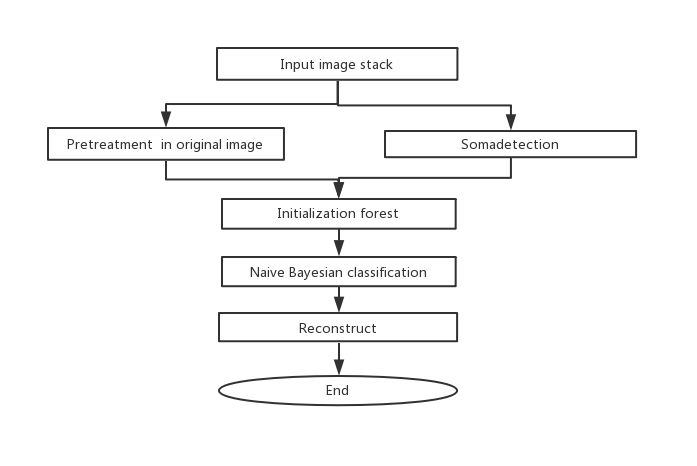
\includegraphics[width=\textwidth]{1.png}
\caption{method overview.} \label{fig1}
\end{figure}

\subsection{Pretreament}
Since the image acquired by v3d has more noise, we use a Gaussian filter to smooth the image, which can remove noise better.
Gaussian LowPassFilter is a linear smoothing filter whose transfer function is a Gaussian function. Also because the Gaussian function is a density function of a normal distribution. Therefore, a Gaussian low-pass filter is very effective for removing noise that obeys a normal distribution.
\begin{equation}
I_{\sigma}=I*G_{\sigma}
\end{equation}
Gaussian function prototype:
\begin{equation}
G_\sigma(x,y,z)=\frac{1}{{2\pi}^{\frac{3}{2}} \delta^3}e^{- \frac{x^2 +y^2+z^2}{2\delta^2}}
\end{equation}

Where I makes the original image, $\sigma$ is the operator of the filter, $I_\sigma$ is the filtered image.
\subsection{Somadetection}
Normally, our reconstruction work starts from the neuronal cell body, so the detection and localization of the cell body is an important part of the automatic reconstruction of neurons. In general, the cell body itself is brighter and farther away from the background area, so we can use the gray scale distance shift (GSDT) to complete the detection of the cell body.

\begin{itemize}
	\item In the first step, the image is foregrounded and segmented using an adaptive threshold segmentation algorithm (OTSU).
	\item In the second step, each voxel maintains its own state value, wherein the state of the background point is set to ALIVE, the state value of the former attraction is set to FAR, and the value of the former attraction is initialized to infinity.
	\item The third step is to initialize the edge points. Select a point in the point with the status ALIVE, change the background point of its 26 neighborhoods to the status value TRAIL, and put it into a queue Q.
	\item In the fourth step, the point y is taken out in the queue Q, and 26 points x around y are calculated, and x is calculated according to the following formula. If the value of x is updated, it is judged whether it is already in the queue, if not, then Put it in the queue. Loop iteration through this step until queue Q is empty.
	\begin{equation}
	d\{x\}=min\{d(x),d(y)+e(x,y)\}
	\end{equation}
	\begin{equation}
	e(x,y)=||x-y||*I(y)
	\end{equation}
	Where I(x) represents the pixel value of the x point, and d(x) represents the shortest weighted distance value of the current point of the x point from the background point.
	\item In the fifth step, the $d(x_i)$ is sorted, the first n maximum values are selected, and the kmeans algorithm is used for clustering, and the clustering category k is selected according to the Parametric Bootstrap method.
	\item In the sixth step, the center of the k categories is output, that is, the position of all the detected cell bodies.
\end{itemize}


\subsection{Forest}
In the previous work, whether it is the single source shortest path of the app or the initial reconstruction method of the app2 based on FM, it is a reconstruction method for a single neuron. In this step, we perform initialization and reconstruction of multiple root nodes.
\begin{itemize}
	\item In the first step, the neuron cell body node $s_i$ is sequentially added to the queue Q.
	\item In the second step, the first cell in the queue, $s_i$, is taken as the root node with $s_i$ as the root node. Based on the FM framework [peng], an initial reconstruction is performed, and the minimum distance of each voxel to the cell node is recorded as $d_{ Ij}$
	\item In the third step, repeat the second step until the queue Q is empty.
\end{itemize}
Where $s_i$ represents the i-th soma point, and $d_i(v)$ represents the shortest path of the voxel $v$ in the tree to $s_i$
\subsection{Naive Bayesian classification}

The core idea of mutil-tracer is based on the Bayesian classifier. In neuron reconstruction, a certain voxel can only belong to a certain neuron cell, which is determined by the biological morphology of the neuron. However, when there are multiple neurons in space, it is not certain which voxel belongs to the voxel in space. Therefore, we need to use the local image data to re-enter the voxel attribution.
There are multiple neuron cells in the space: $S_i(x_i^1, x_i^2,...)$ where $S_i$ represents the i-th neuron cell, and $x_i^j$ represents the i-th neuron j features. The i-th voxel is characterized by $V_i$, which is a vector, and the probability that the i-th voxel belongs to the j-th neuron can be expressed as

\begin{equation}
P(S|V)=\frac{P(S)P(V|S)}{P(V)}=\frac{P(s)}{p(v)}\sum_{i=1}^ {d}P(V^i|S)
\end{equation}



Where d is the number of attributes and $v^i$ is the value of voxel V above the i-th attribute. Therefore, the Bayesian criteria based on this are:
\begin{equation}
H_{nb}{(V)}=\mathop{\arg\max}_{(V belong )}P(S)\sum_{i=1}^d p(v_i|s)
\end{equation}

Where 
\begin{equation}
\sum_{i=1}^n P(S_i|V_i)=1
\end{equation}

The category of the i-th voxel $V_i$
\begin{equation}
L(S)=\mathop{\arg\max}_{S}P(S|V_i)
\end{equation}

In the Bayesian classifier, P is multiply, the efficiency is too low, we can use the greedy method.

\begin{equation}
Label(v)=\mathop{\arg\min}_{i}C_i(v)
\end{equation}

Where $Label(v)$ denotes the label of voxel V, and $C_i(v)$ the cost of dividing voxel V into the i-th neuron cell.
Here, we can use the $d_i(v)$ approximation of the previous step instead of $C_i(v)$


\subsection{Reconstuction}
Based on the spatial voxel partitioning, we can use any published reconstruction methods, including but not limited to APP1, APP2, etc.

\section{EXPERIMENTAL RESULTS}
\subsection{Experiment data}
Our data set is the neurons of 302 mouse brains, 124 of which are from the mouse brain numbered 17302 and 178 from the mouse brain numbered 18454. These neurons have been the gold standard for manual reconstruction. We cut it into 512x512x512 image blocks and tested the neuron reconstruction algorithm. The number of image blocks in multiple neuron cell bodies in the same field of view is 93, of which 27 are from 17302 and 66 are from 18454. We mainly study the quality of these 93 multi-neuron reconstructions.
\subsection{Experimental Setup}
We compared the Multi-tracer with several leading semi-automatic reconstruction methods in the field, including APP, APP2, and through semi-automatic and manual integration.
The real gold reconstruction standard. Calculate the difference score between the automatic reconstruction result and the gold standard. These scores were previously defined by Peng et al.



\begin{figure}[htbp]
	\centering
	\subfigure[17302-ID(8)]{
		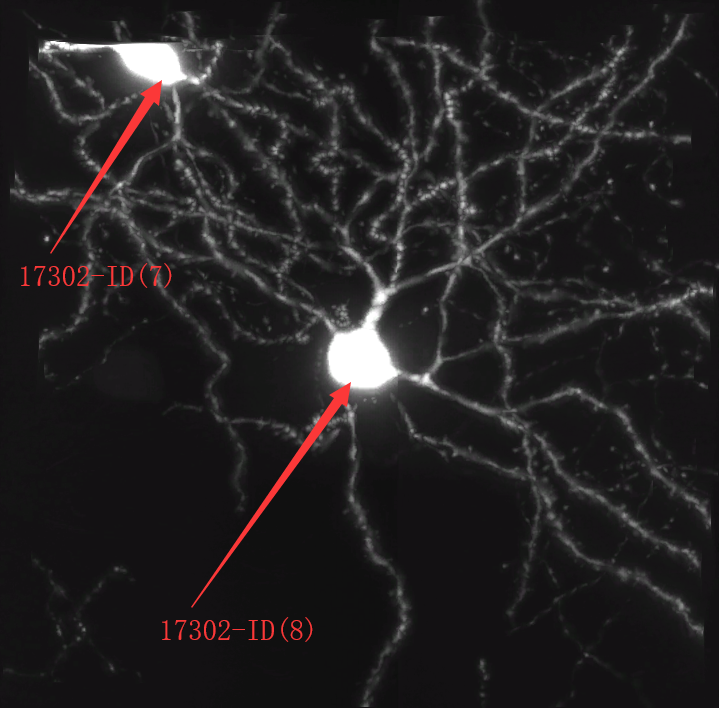
\includegraphics[width=2.75cm]{17302-ID(8).png}
		%\caption{fig1}
	}
	\subfigure[Ground Truth]{
	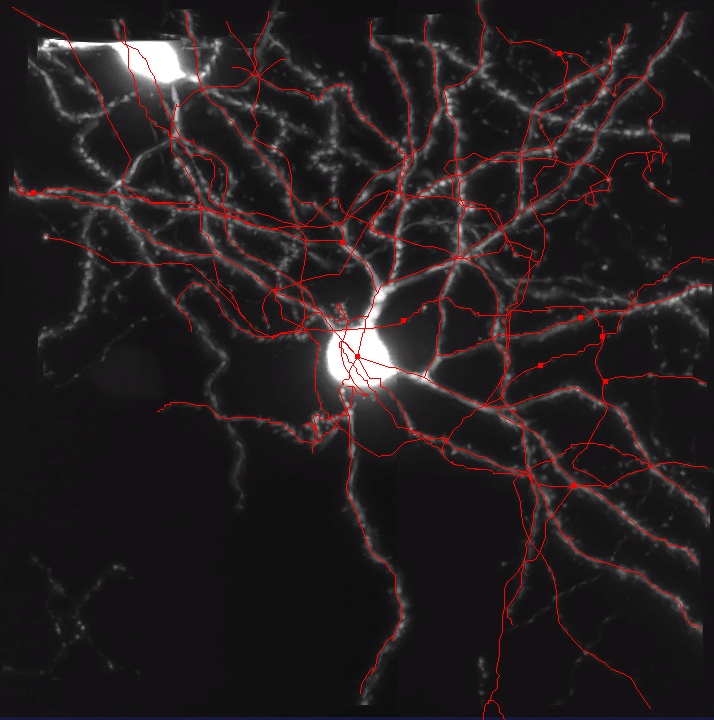
\includegraphics[width=2.75cm]{17302-ID(8)TRUE.png}
	}
	\subfigure[Multi-Tracer]{
		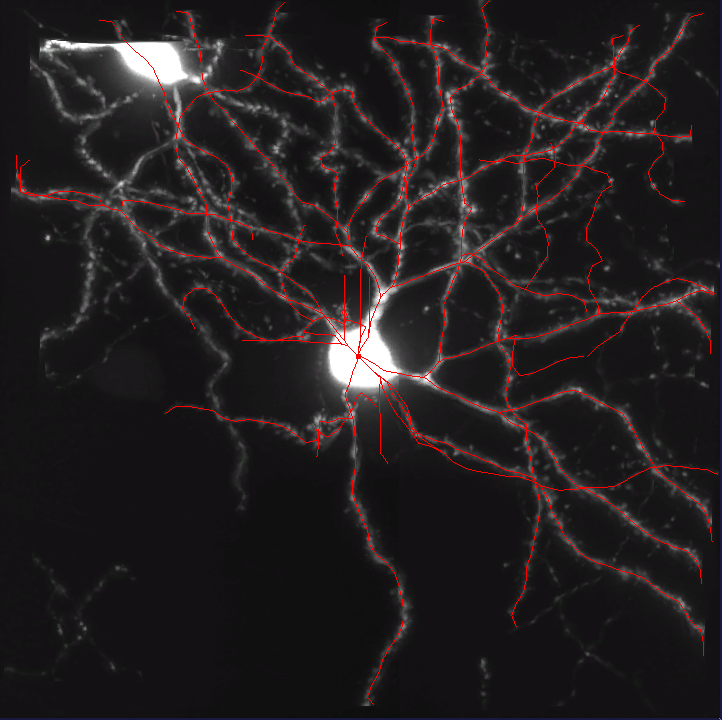
\includegraphics[width=2.75cm]{17302-ID(8)MULTI-TRACER.png}
	}
	\subfigure[APP2]{
		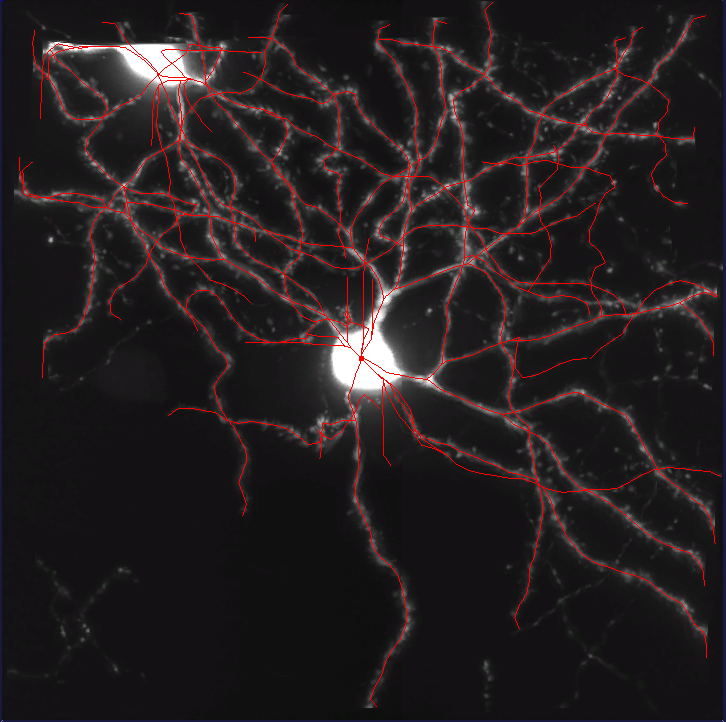
\includegraphics[width=2.75cm]{17302-ID(8)APP2.png}
	}

	\subfigure[17302-ID(87)]{
		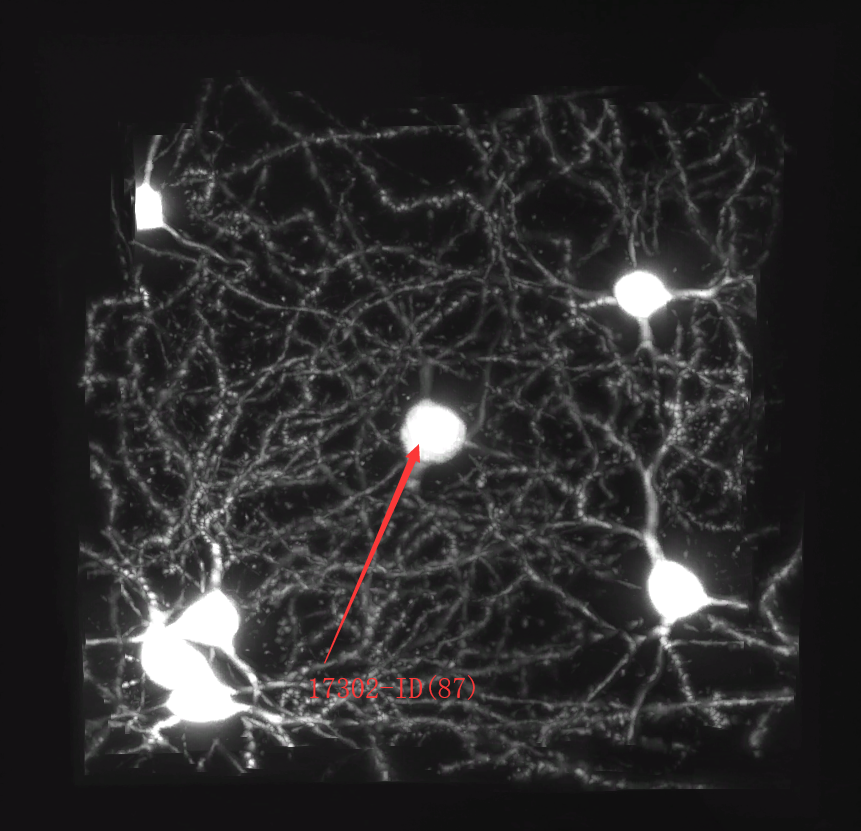
\includegraphics[width=2.75cm]{17302-ID(87).png}
		%\caption{fig1}
	}
	\subfigure[Ground Truth]{
		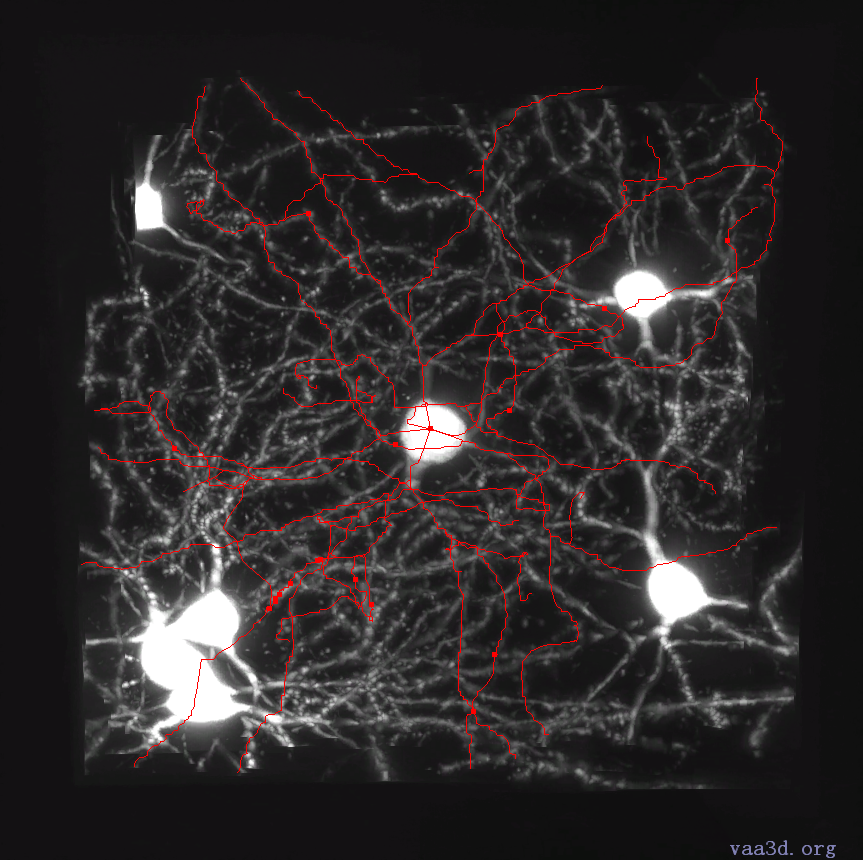
\includegraphics[width=2.75cm]{17302-ID(87)TRUE.png}
	}
	\subfigure[Multi-Tracer]{
		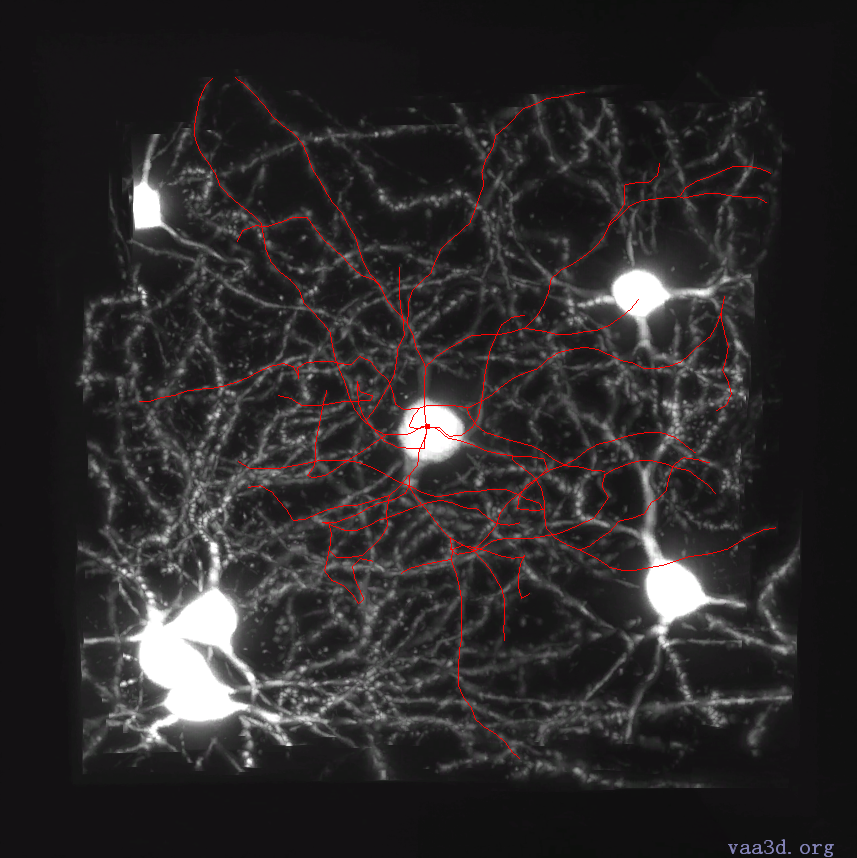
\includegraphics[width=2.75cm]{17302-ID(87)MULTI-TRACER.png}
	}
	\subfigure[APP2]{
		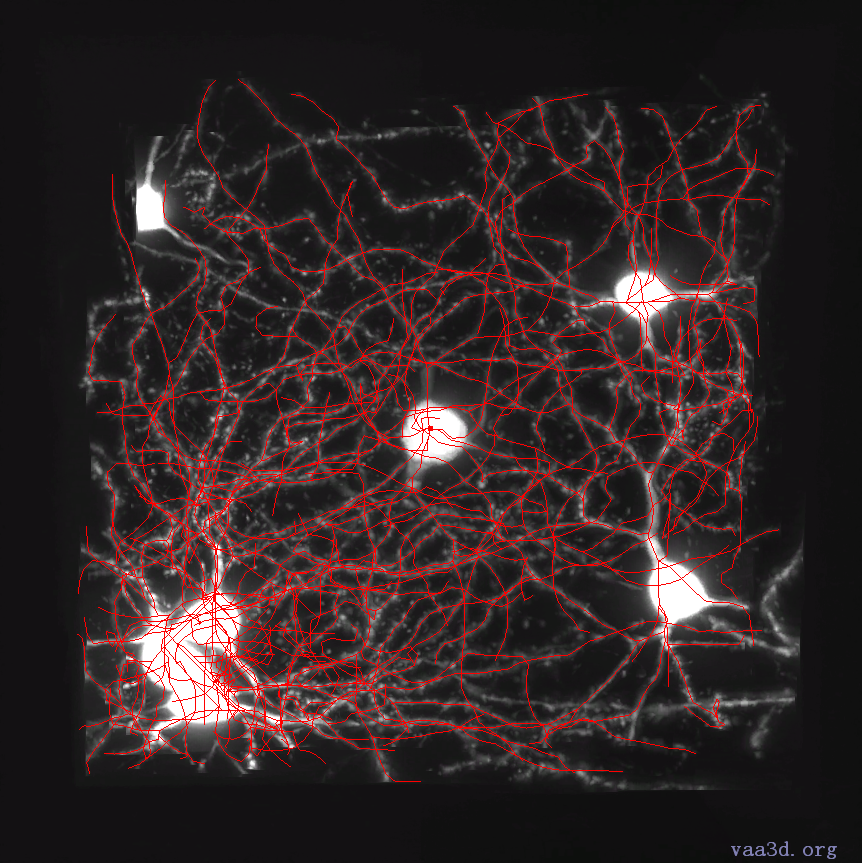
\includegraphics[width=2.75cm]{17302-ID(87)APP2.png}
	}

	\subfigure[17302-ID(8)]{
		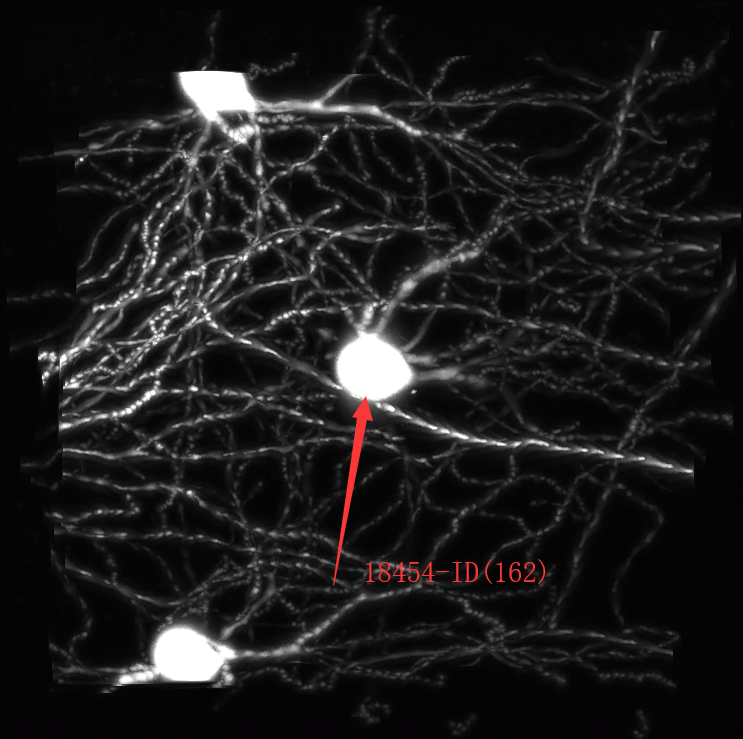
\includegraphics[width=2.75cm]{18454-ID(162).png}
		%\caption{fig1}
	}
	\subfigure[Ground Truth]{
		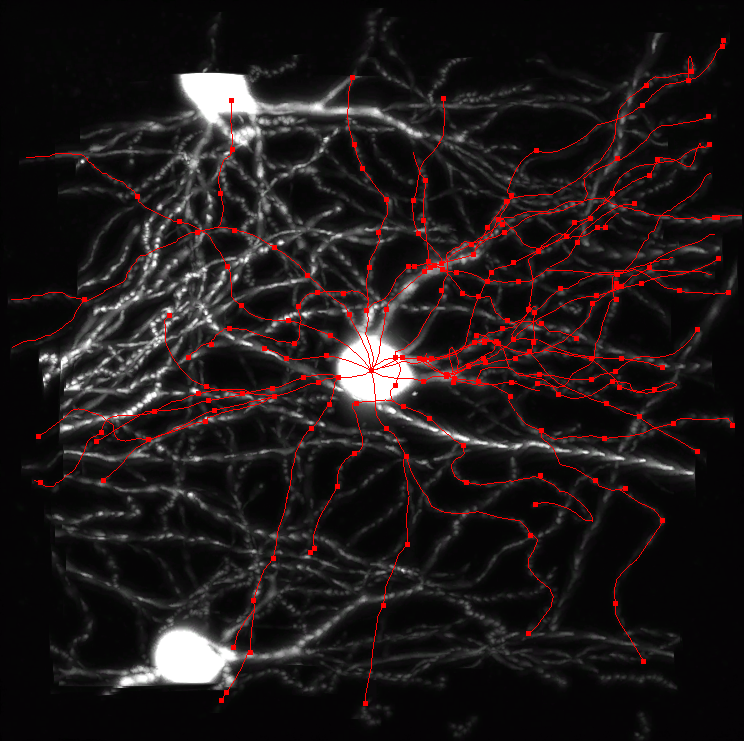
\includegraphics[width=2.75cm]{18454-ID(162)TRUE.png}
	}
	\subfigure[Multi-Tracer]{
		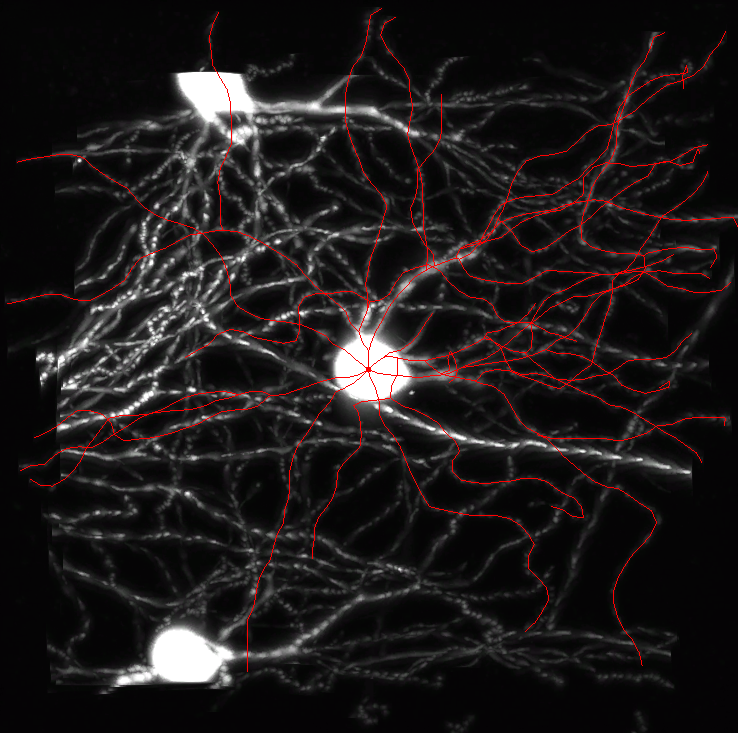
\includegraphics[width=2.75cm]{18454-ID(162)MULTI-TRACER.png}
	}
	\subfigure[APP2]{
		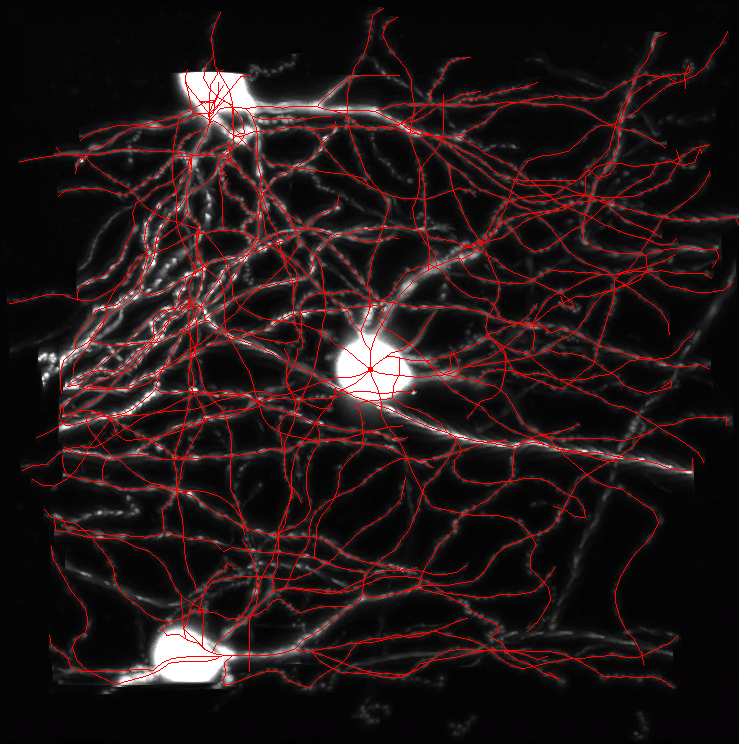
\includegraphics[width=2.75cm]{18454-ID(162)APP2.png}
	}
	
	
	\subfigure[]{
		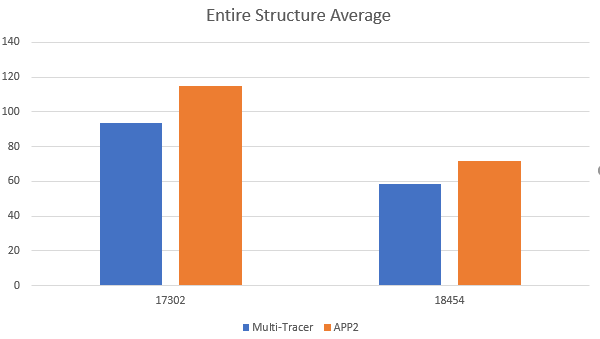
\includegraphics[width=3.7cm]{Structure.png}
	}
	\subfigure[]{
		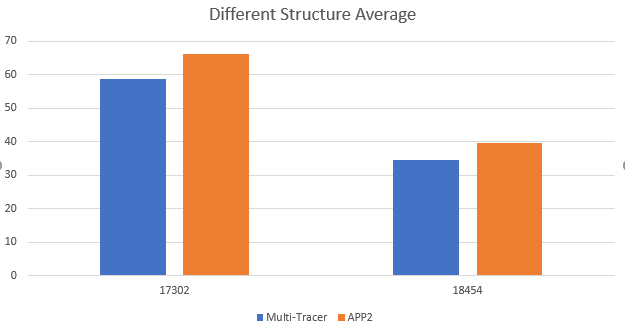
\includegraphics[width=3.7cm]{diffStructure.png}
	}
	\subfigure[]{
	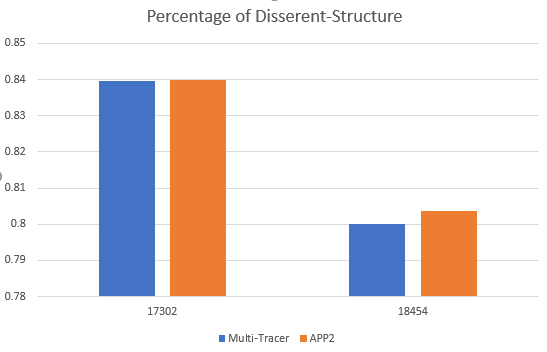
\includegraphics[width=3.7cm]{percentage.png}
	}

	\caption{The first row to the third row correspond to the reconstruction results of the 17302-ID (8), 17302-ID (87), and 18454-ID (162) neurons, respectively. The fourth line is the three average difference scores of 27 neurons of 17302 and 66 neurons of 18454.}
\end{figure}

It can be found that in a dense area of neurons, that is, when there are multiple neurons in one field of view, APP2 will reach other neuron nodes from the current neurons, resulting in large-scale error reconstruction. Multi-Tracer has already divided the voxels in space based on the Bayesian classifier before the reconstruction work, thus avoiding similar errors and not erroneously tracking other neuron nodes.

You can see even further
Multi-Tracer is superior to APP2 in three aspects: entire-structure-average, differen-structure-average, and percent of different-structure.

\subsection{Futher experiment}
Glial cells are similar in morphology to neuronal cell bodies, which is a major obstacle to the automatic reconstruction of neurons in the past, but we can cope with this situation by using Multi-tracer.

\begin{figure}[htbp]
	\centering
	\subfigure[17302-ID(87)]{
		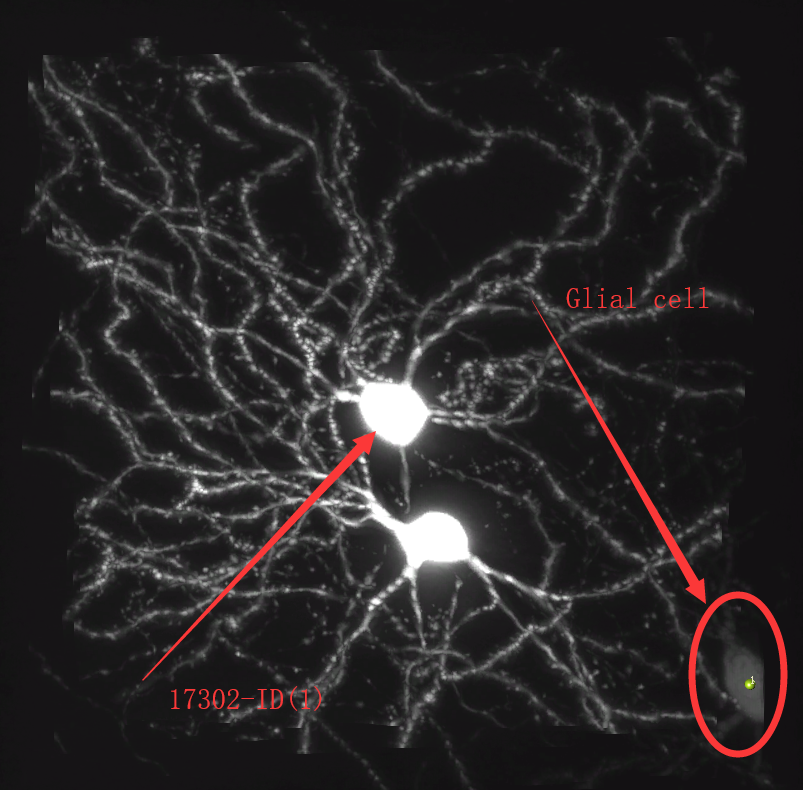
\includegraphics[width=5.5cm]{17302-ID(1).png}
		%\caption{fig1}
	}
	\subfigure[Ground Truth]{
		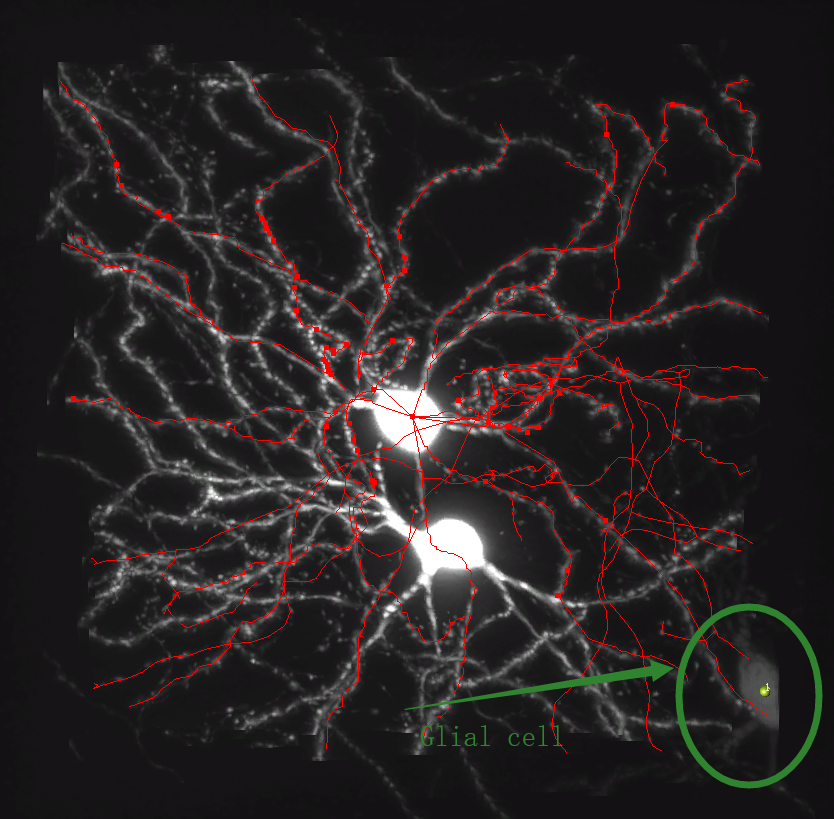
\includegraphics[width=5.5cm]{17302-ID(1)TRUE.png}
	}

	\subfigure[APP2]{
		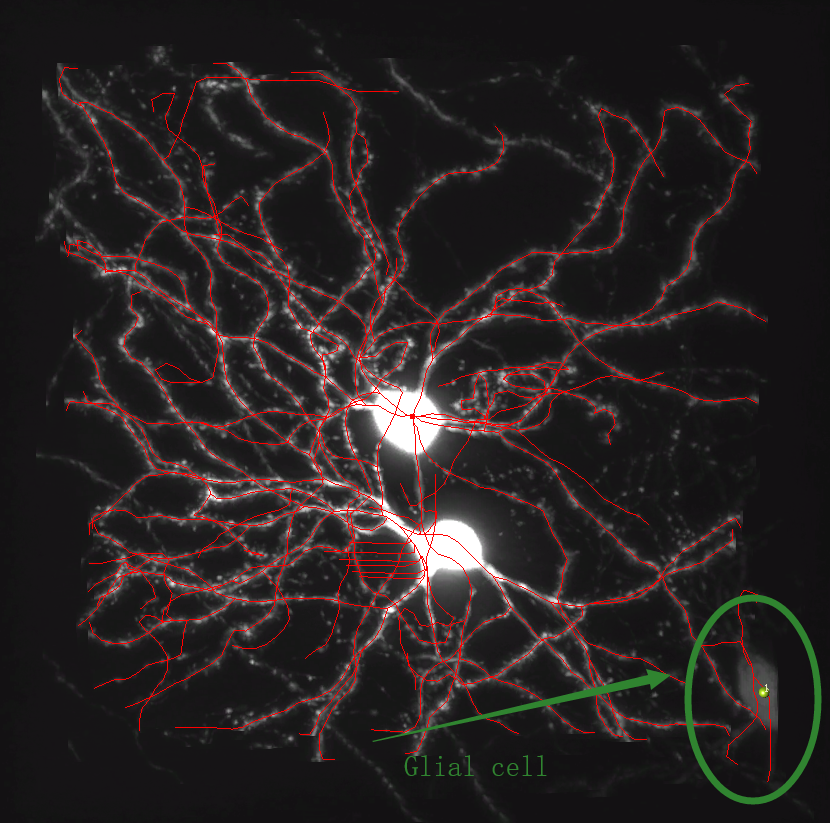
\includegraphics[width=5.5cm]{17302-ID(1)APP2.png}
	}
	\subfigure[APP2-GivenGlial]{
		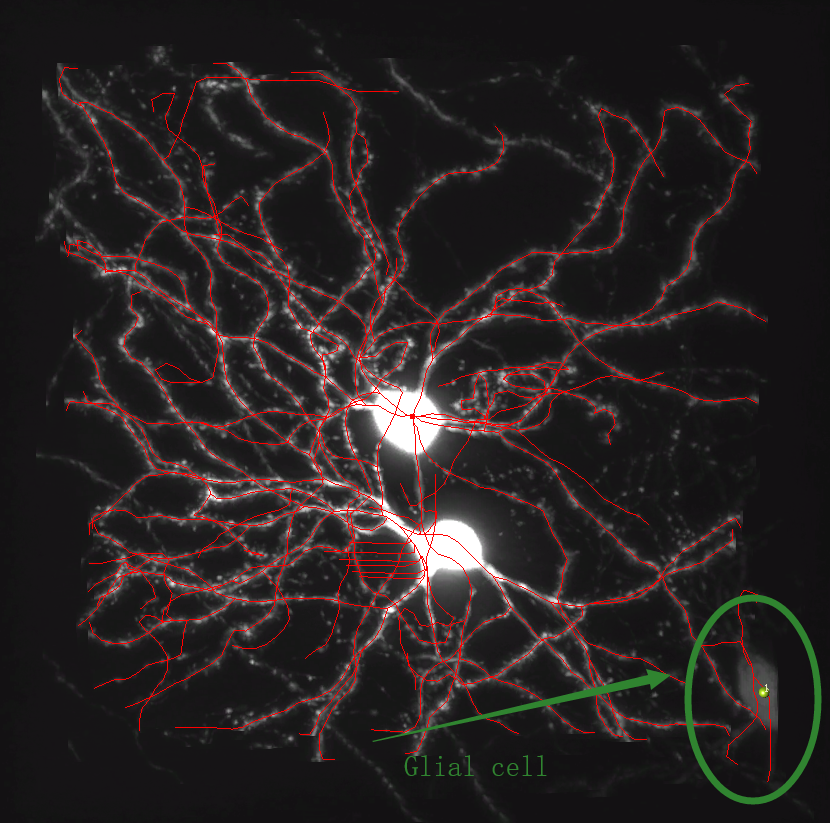
\includegraphics[width=5.5cm]{17302-ID(1)APP2-GivenGlial.png}
	}
	
	\subfigure[MULTI-TRACER]{
		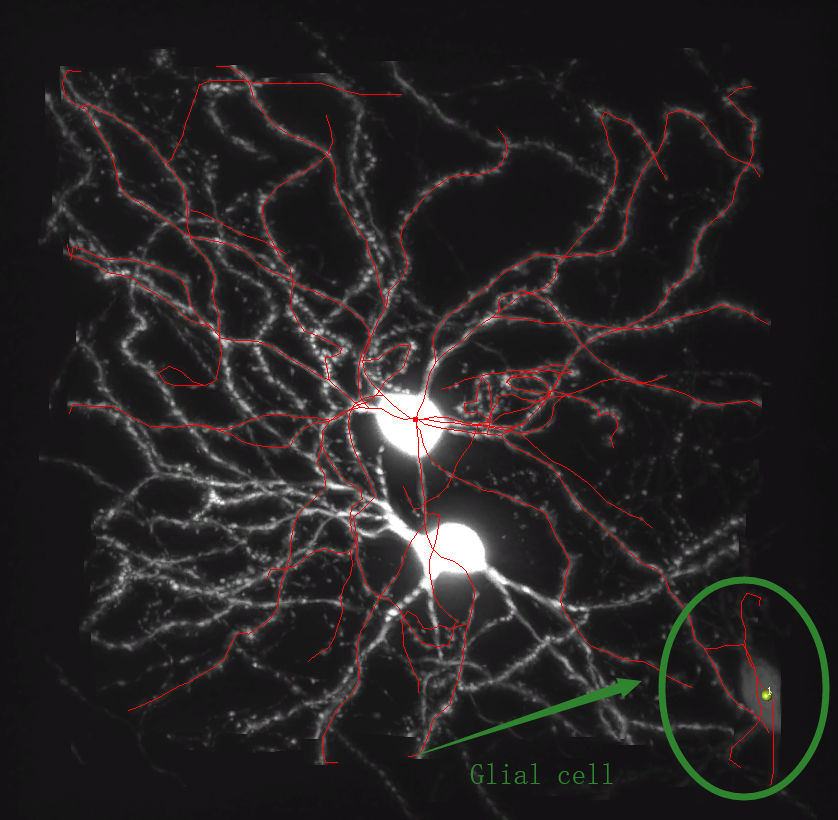
\includegraphics[width=5.5cm]{17302-ID(1)MULTI-TRACER.png}
	}
	\subfigure[MULTI-TRACER-GivenGlial]{
	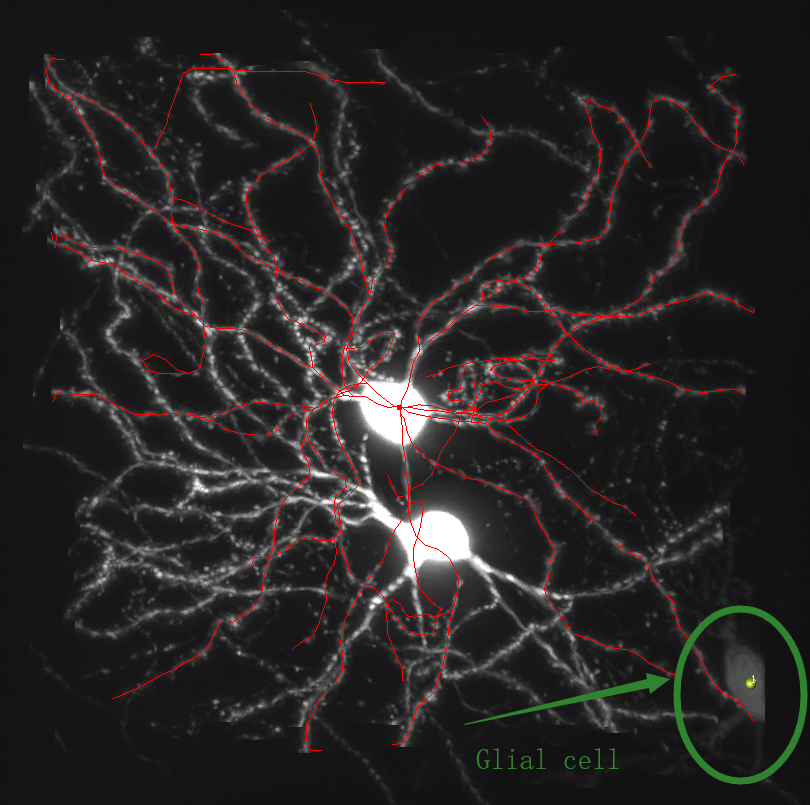
\includegraphics[width=5.5cm]{17302-ID(1)MULTI-TRACER-GivenGlial.png}
	}

	
	
	\caption{(a) is the local map of neuron No. 1 in the brain of mouse 17302, (b) is the manual reconstruction, that is, the standard is changed, (c) (e) is the reconstruction result of APP2 and Multi-Tracer, respectively, (d) (f ) is the result of reconstruction of APP2 and Multi-Tracer after the location of the glial cells.}
\end{figure}

When the location of the glial cells is given, our algorithm can avoid erroneous tracking of glial cells. So far we can combine the detection of glial cells and the detection of neuronal cell bodies into one category, which greatly simplifies reconstruction. Hard work


%
% ---- Bibliography ----
%
% BibTeX users should specify bibliography style 'splncs04'.
% References will then be sorted and formatted in the correct style.
%
% \bibliographystyle{splncs04}
% \bibliography{mybibliography}
%
\begin{thebibliography}{8}
\bibitem{ref_article1}
Author, F.: Article title. Journal \textbf{2}(5), 99--110 (2016)

\bibitem{ref_lncs1}
Author, F., Author, S.: Title of a proceedings paper. In: Editor,
F., Editor, S. (eds.) CONFERENCE 2016, LNCS, vol. 9999, pp. 1--13.
Springer, Heidelberg (2016). \doi{10.10007/1234567890}

\bibitem{ref_book1}
Author, F., Author, S., Author, T.: Book title. 2nd edn. Publisher,
Location (1999)

\bibitem{ref_proc1}
Author, A.-B.: Contribution title. In: 9th International Proceedings
on Proceedings, pp. 1--2. Publisher, Location (2010)

\bibitem{ref_url1}
LNCS Homepage, \url{http://www.springer.com/lncs}. Last accessed 4
Oct 2017
\end{thebibliography}
\end{document}
